\documentclass[10pt]{article}
\usepackage[a4paper]{geometry}
\usepackage{fullpage}
\usepackage[T1]{fontenc}
\usepackage[utf8]{inputenc}
\usepackage{graphicx}
\usepackage{mathpazo}
\pagenumbering{gobble}
\usepackage{siunitx}
\DeclareSIUnit\voltampere{VA}
\DeclareSIUnit\kWh{kWh}
\usepackage{amsmath}
\usepackage[spanish]{babel}
\usepackage{steinmetz}
\usepackage{enumitem}

\begin{document}

\title{Problemas de Electrotecnia}

\date{}

\author{Oscar Perpiñán Lamigueiro}

\maketitle

\section*{Corriente Continua}

Un generador cuya fuerza electromotriz es de \SI{120}{V} y resistencia interna \SI{0.2}{\ohm}, entrega una corriente de \SI{20}{\ampere} a un motor situado a \SI{300}{\meter} de distancia y de resistencia interna \SI{0.5}{\ohm}. La línea es de cobre de resistividad $\SI{17.24}{\milli\ohm\milli\meter\squared\per\meter}$. Sabiendo que el motor absorbe \SI{10.2}{\kWh} en 5 horas, hallar: 
\begin{enumerate}
\item Fuerza contraelectromotriz del motor.
\item Sección de los conductores.
\item Balance general de potencias.
\item Rendimiento del motor, del generador, de la línea y rendimiento total.
\end{enumerate}

\subsection*{Solución}

\begin{center}
  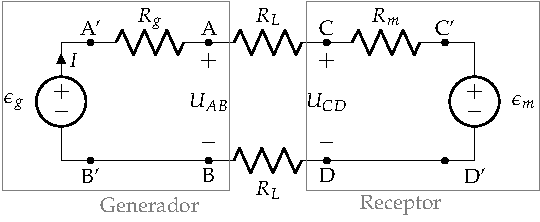
\includegraphics{../figs/circuito_lkv}
\end{center}

La energía absorbida por el motor nos permite calcular la potencia del mismo, teniendo en cuenta el período de cálculo de la energía:
\[
  E_{motor} = \SI{10.2}{\kWh} \rightarrow P_{Tm} = \frac{10.2}{5} = \SI{2.04}{\kilo\watt}
\]

Este resultado es la potencia absorbida, es decir, incluye las pérdidas del motor (modeladas por la resistencia interna)

\[
  P_{Tm} = P_m + I^2 \cdot R_m \rightarrow P_m = 2040 - 20^2 \cdot 0.5 = \SI{1840}{\watt}
\]

Por tanto,

\[
  P_m = \epsilon_m \cdot I \rightarrow \epsilon_m = \SI{92}{\volt}
\]

Para calcular la sección de los conductores, dado que sabemos la resistividad, la longitud, y la corriente que circula, necesitamos obtener la caída de tensión en la línea.

La tensión a la entrada del motor es:

\[
  U_{CD} = I \cdot R_m + \epsilon_m = \SI{102}{\volt}
\]

La tensión a la salida del generador es:


\[
  U_{AB} = \epsilon_g - I \cdot R_g = \SI{116}{\volt}
\]

Por tanto, en la línea hay una caída de $U_{AB} - U_{CD} = \SI{14}{\volt}$ debida al paso de la corriente. Dado que los dos conductores son iguales, la caída de tensión es la misma en cada uno de ellos:

\[
  U_{AC} = \SI{7}{\volt} = I \cdot R_L \rightarrow R_L = \SI{0.35}{\ohm}
\]

Con la fórmula de la resistencia obtenemos la sección de los conductores:

\[
  R_L = \rho \cdot \frac{L}{S} \rightarrow S = \SI{14.77}{\milli\meter\squared}
\]

Habría que elegir el valor normalizado inmediatamente superior que, en este caso, es $S = \SI{16}{\milli\meter\squared}$.


El balance de potencias es:

\begin{itemize}
\item El generador produce $\epsilon_g \cdot I = \SI{2400}{\watt}$, de los que entrega $U_{AB} \cdot I = \SI{2320}{\watt}$ al circuito, y disipa $R_g \cdot I^2 = \SI{80}{\watt}$ internamente.
\item La línea recibe $U_{AB} \cdot I = \SI{2320}{\watt}$, disipa $2 \cdot R_L \cdot I^2 = \SI{280}{\watt}$ y entrega $U_{CD} \cdot I = \SI{2040}{\watt}$ al motor.
\item El motor recibe $U_{CD} \cdot I = \SI{2040}{\watt}$, disipa $R_m \cdot I^2 = \SI{200}{\watt}$ y utiliza $\epsilon_m \cdot I = \SI{1840}{\watt}$.  
\end{itemize}

Por tanto, los rendimientos de cada parte del circuito son:

\[
  \eta_m = \frac{P_{util}}{P_{absorbida}} = \frac{\epsilon_m \cdot I}{U_{CD} \cdot I} = 0.902
\]

\[
  \eta_g = \frac{P_{entregada}}{P_{generada}} = \frac{U_{AB} \cdot I}{\epsilon_g \cdot I} = 0.97
\]

\[
  \eta_{linea} = \frac{P_{salida}}{P_{entrada}} = \frac{U_{CD} \cdot I}{U_{AB} \cdot I} = 0.88
\]

\[
  \eta_t = \frac{P_{util}}{P_{generada}} = \frac{\epsilon_m \cdot I}{\epsilon_g \cdot I} = 0.77
\]

\clearpage

\section*{Corriente Alterna Monofásica}

Un generador de corriente alterna ($f = \SI{50}{\hertz}$) alimenta una instalación eléctrica a través de una línea de cobre ($\rho = \SI{0.017}{\ohm\milli\meter\squared\per\meter}$) de $\SI{25}{\milli\meter\squared}$ de sección. La instalación eléctrica está compuesta por un motor de $S_m = \SI{10}{\kilo\voltampere}$ y $\mathrm{fdp} = 0.8$, una instalación de alumbrado fluorescente de $P_f = \SI{800}{\watt}$ y $\mathrm{fdp} = 0.9$, y diversas cargas electrónicas con una potencia conjunta $P_e = \SI{540}{\watt}$ y $\mathrm{fdp} = 0.5$ en retraso.

Suponiendo que las cargas trabajan a su tensión nominal de $\SI{230}{\volt}$ y que están situadas a $\SI{100}{\meter}$ del generador, calcule:

\begin{enumerate}
\item Triángulo de potencias total de las cargas ($P_T$, $Q_T$, $S_T$) y factor de potencia.
\item Valor eficaz de la corriente que circula por la línea.
\item Potencia disipada en la línea.
\item Triángulo de potencias del generador ($P_g$, $Q_g$, $S_g$) y factor de potencia.
\item Valor eficaz de la tensión de salida del generador.
\item Capacidad del banco de condensadores a instalar en bornes de la carga necesario para reducir la corriente que circula por la línea a un valor de $\SI{45}{\ampere}$.
\end{enumerate}

Independientemente del resultado obtenido, suponga que la capacidad instalada es $C = \SI{172}{\micro\farad}$. En estas condiciones, calcule:
\begin{enumerate}[resume]
\item Potencia aparente de las cargas (incluyendo al banco de condensadores)
\item Valor eficaz de la corriente que circula por la línea y potencia disipada en la misma.
\item Triángulo de potencias del generador y factor de potencia.
\item Tensión de trabajo del generador.
\end{enumerate}

\subsection*{Solución}

\begin{enumerate}
\item Triángulo de potencias total de las cargas ($P_T$, $Q_T$, $S_T$)
  y factor de potencia.

  Motor:
  \begin{align*}
    P_m &= \SI{8000}{\watt}\\
    Q_m &= \SI{6000}{\voltampere}_r\\
  \end{align*}

  Alumbrado
  \begin{align*}
    P_f &= \SI{800}{\watt}\\
    Q_f &= \SI{387.5}{\voltampere}_r\\
  \end{align*}

  Cargas Electrónicas
  \begin{align*}
    P_e &= \SI{540}{\watt}\\
    Q_e &= \SI{935.3}{\voltampere}_r\\
  \end{align*}

  Total (Teorema de Boucherot)
  \begin{align*}
    P_T &= P_m + P_f + P_e = \SI{9340}{\watt}\\
    Q_T &= Q_m + Q_f + Q_e = \SI{7322.8}{\voltampere}_r\\
  \end{align*}

  Por tanto, $S_T = \SI{11868.4}{\voltampere}$ y
  $\mathrm{fdp}_T = 0.787$.

\item Valor eficaz de la corriente que circula por la línea.
  \[
    I = \frac{S_T}{U} = \frac{11868.4}{230} = \SI{51.6}{\ampere}
  \]

\item Potencia disipada en la línea.

  \begin{align*}
    R &= \SI{0.068}{\ohm}\\
    P_L &= 2 \cdot I^2 \cdot R = \SI{362.1}{\watt}
  \end{align*}

\item Triángulo de potencias del generador ($P_g$, $Q_g$, $S_g$) y
  factor de potencia.


  \begin{align*}
    P_g &= P_T + P_L = \SI{9702.1}{\watt}\\
    Q_g &= Q_T = \SI{7322.8}{\voltampere}_r\\
    S_g &= \SI{12155.4}{\voltampere}\\    
    \mathrm{fdp} &= 0.798
  \end{align*}

\item Valor eficaz de la tensión de salida del generador.

  \[
    U_g = \frac{S_g}{I} = \SI{235.6}{\volt}
  \]

\item Capacidad del banco de condensadores a instalar en bornes de la
  carga necesario para reducir la corriente que circula por la línea a
  un valor de $\SI{45}{\ampere}$.

  Si la corriente en línea se reduce a $\SI{45}{\ampere}$ la potencia
  aparente resultante en cargas (incluyendo al condensador) es
  $S'_T = 230 \cdot 45 = \SI{10350}{\voltampere}$. Por tanto,
  $Q'_T = \SI{4459.5}{\voltampere}_r$. Así, es necesario instalar un
  banco de condensadores que aporte
  $Q_c = Q_T - Q'_T = \SI{2863.3}{\voltampere}_r$.

\[
  C = \frac{Q_c}{\omega U^2} = \SI{172.3}{\micro\farad}
\]

  
\end{enumerate}

Independientemente del resultado obtenido, suponga que la capacidad
instalada es $C = \SI{172}{\micro\farad}$. En estas condiciones,
calcule:
\begin{enumerate}[resume]
\item Potencia aparente de las cargas (incluyendo al banco de
  condensadores)
  \[
    S'_T = \sqrt{P^2_T + Q'^2_T} = \SI{10350.1}{\voltampere}
  \]

\item Valor eficaz de la corriente que circula por la línea y potencia
  disipada en la misma.
  \[
    I' = \frac{S'_T}{U} = \SI{45}{\ampere}
  \]

\[
  P'_L = 2 \cdot I'^2 \cdot R = \SI{275.4}{\watt}
\]

\item Triángulo de potencias del generador y factor de potencia.
  \begin{align*}
    P'_g &= P_T + P'_L = \SI{9615.4}{\watt}\\
    Q'_g &= Q'_T = \SI{4459.5}{\voltampere}_r\\
    S'_g &= \SI{10599.2}{\voltampere}\\    
  \end{align*}

\item Tensión de trabajo del generador.
  \[
    U'_g = \frac{S'_g}{I'} = \SI{235.5}{\volt}
  \]
\end{enumerate}

\clearpage
\section*{Corriente Alterna Trifásica}

Una plantación agrícola emplea dos bombas sumergibles para extraer
agua de un pozo y transportarla a través de un sistema de riego por
goteo. Estas dos bombas están alimentadas a \SI{400}{\volt} por una
línea trifásica en secuencia de fases directa y frecuencia
$\SI{50}{\hertz}$. Una de las bombas funciona con un motor trifásico
de $\SI{30}{\kilo\watt}$ y factor de potencia de 0.78. La otra bomba
trabaja con un motor de $\SI{7.5}{\kilo\watt}$ y factor de potencia de
0.67.  La línea que alimenta estas dos bombas es resistiva, con
resistividad $\rho = \SI{0.017}{\ohm\milli\meter\squared\per\meter}$,
longitud de \SI{300}{m} y una sección de
\SI{35}{\milli\meter\squared}.
 
\begin{enumerate}
\item Calcula el triángulo de potencias (potencia activa, reactiva, y
  aparente) de cada carga, y total de las cargas (a la salida de la
  línea).
\item Calcula el \textbf{valor eficaz} de la corriente de línea de
  cada carga, y total.
\item Calcule el triángulo de potencias a la entrada de la línea.
\item Calcule el \textbf{valor eficaz} de la tensión a la entrada de
  la línea.
\item Calcule los condensadores que se deben conectar a la salida de
  la línea para mejorar el factor de potencia del sistema hasta la
  unidad. Indique el modo de conexión.
\end{enumerate}

Una vez conectados los condensadores del último apartado:
\begin{enumerate}[resume]
\item Calcule el \textbf{valor eficaz} de la corriente de línea total.
\item Calcule el triángulo de potencias a la entrada de la línea.
\item Calcule el \textbf{valor eficaz} de la tensión a la entrada de
  la línea.
\end{enumerate}

\subsection*{Solución}

Las potencias de cada carga son:
\begin{align*}
  P_1 &= \SI{30}{\kilo\watt}\\
  Q_1 &= P_1\tan \theta_1 = \SI{24.06}{\kilo\voltampere}_r\\
  S_1 &= \SI{38.46}{\kilo\voltampere}\\
  P_2 &= \SI{7.5}{\kilo\watt}\\
  Q_2 &= P_2 \tan \theta_2 = \SI{8.31}{\kilo\voltampere}_r\\
  S_2 &= \SI{11.19}{\kilo\voltampere}
\end{align*}

Aplicando Boucherot, el triángulo de potencias total es:
\begin{align*}
  P_T &= \SI{37.5}{\kilo\watt}\\
  Q_T &= \SI{32.37}{\kilo\voltampere}_r\\
  S_T &= \sqrt{P_T^2 + Q_T^2} = \SI{49.54}{\kilo\voltampere}
\end{align*}

Por tanto, el ángulo de la impedancia global es:

\[
  \tan(\theta) = \frac{Q_T}{P_T} = 0.8632 \rightarrow \theta =
  \ang{40.8}
\]

Las corrientes en cada carga son:

\begin{align*}
  I_1 &= \frac{S_1}{\sqrt{3} U} = \SI{55.51}{\ampere}\\
  I_2 &= \frac{S_2}{\sqrt{3} U} = \SI{16.15}{\ampere}
\end{align*}

La corriente total es:
\[
  I = S_T /{\sqrt{3} U} = \SI{71.5}{\ampere}
\]

La resistencia de la línea (una resistencia por cada conductor) es:

\[
  R_L = \rho L/S = \SI{0.146}{\ohm}
\]

La potencia activa disipada en la línea es:

\[
  P_L = 3 \cdot I^2 R_L = \SI{2234.8}{\watt}
\]

Por tanto, la potencia a la entrada de la línea es:

\begin{align*}
  P_g &= P_L + P_T = \SI{39.73}{\kilo\watt}\\
  Q_g &= Q_T = \SI{32.33}{\kilo\voltampere}_r\\
  S_g &= \SI{51.22}{\kilo\voltampere}
\end{align*}

Y la tensión a la salida del generador (entrada de la línea) es:

\[
  U_g = \frac{S_g}{\sqrt{3} I} = \SI{413.64}{\volt}
\]

Para mejorar el factor de potencia a la unidad en las cargas, se
necesita una batería de condensadores conectados en triángulo en las
cargas (a la salida de la línea). Cada uno de los tres condensadores
debe tener una capacidad de:

\[
  C = \frac{Q_T}{3 \omega U^2} = \SI{214.4}{\micro\farad}
\]

Una vez instalada la batería de condensadores, la corriente total a la
salida de la línea es:

\[
  I' = \frac{P_T}{\sqrt{3} U} = \SI{54.13}{\ampere}
\]

La potencia disipada en la línea es ahora:

\[
  P'_L = 3 \cdot I'^2 R_L = \SI{1282.9}{\watt}
\]

Por tanto, el triángulo de potencias a la entrada de la línea es:
\begin{align*}
  P'_g &= \SI{38.78}{\kilo\watt}\\
  Q'_g &= \SI{0}{\kilo\voltampere}_r\\
  S'_g &= \SI{38.78}{\kilo\voltampere}
\end{align*}

Consecuentemente, la tensión a la entrada de la línea es:

\[
  U' = \frac{S'_g}{\sqrt{3} I'} = \SI{413.63}{\volt}
\]

\end{document}





